\subsubsection{Model Evaluation}
	\paragraph{Classification Error}
		\RTheory
		{
			$$\varepsilon = \frac{1}{N}\sum\limits_{n = 0}^N I(\hat{y}_n \neq y_n)$$
		}
		{
			sections/Classification/LogisticRegression/ModelEvaluation/ClassificationError.R
		}
		
	\paragraph{Confusion Matrix}
		\RTheory
		{
			\vspace{0pt}
			
			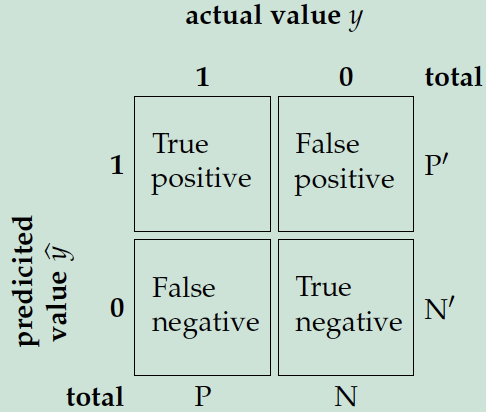
\includegraphics{images/ConfusionMatrix.png}
		}
		{
			sections/Classification/LogisticRegression/ModelEvaluation/ConfusionMatrix.R
		}
		
	\paragraph{Cross Validation}
		Generic method for estimating the classification error without needing extra data.
		\subparagraph{Algorithm}
			\RTheory
			{
				\begin{itemize}
				    \item The \underline{training data} is divided in $k$ groups (folds) of approximately the same size
				    \item First fold is treated as validation set
				    \item The model is fit on the remaining $k-1$ folds
				    \item The classification error $\mathrm{Err}_1$ is calculated
				    \item The process is repeated for the remaining sets, resulting in classification errors $\mathrm{Err}_1, \dots, \mathrm{Err}_k$
				    \item The CV error is computed as: $CV_{(k)} = \frac{1}{k} \sum\limits_{i=1}^k\mathrm{Err}_i$
				\end{itemize}
			}
			{
				sections/Classification/LogisticRegression/ModelEvaluation/CrossValidation.R
			}

		